\documentclass{article}
\usepackage[UTF8]{ctex}
\usepackage{amsmath}
\usepackage{amssymb}
\usepackage{graphicx}
\usepackage{float}
\usepackage{datetime}
\usepackage{geometry}
\usepackage{pythonhighlight}

\geometry{a4paper, top=2.54cm, bottom=2.54cm, left=3.18cm, right=3.18cm}

\author{刘思昀 SLST 2022522011}

\title{General Physics II RLC电路的串联谐振}

\begin{document}

\date{\formatdate{22}{5}{2024}}

\maketitle

\section{测量RLC串联谐振谐振曲线}
\subsection{测量谐振曲线}
选取$R = 10 \Omega$,连接RLC串联电路,先固定信号源输出电压为$1.00V$,随后将示波器切换到XY模式(李萨如图形),调节信号源频率,直到示波器上出现一条直线,此时找到RLC电路的谐振频率为$v_0 = 79.000 kHz$。

将示波器切换到YT模式,调节信号源输出电压,直到示波器上显示整个电路两端的电压为$U_i = 1.00V$,记录电阻R的输出电压$U_R = 696 mV$

之后,改变信号源的频率,每次调节频率后,都需通过调整信号源输出电压,使得示波器上显示整个电路两端的电压为$U_i= 1.00V$,然后记录电阻R的输出电压,得到数据如下:
\begin{figure}[htbp]
    \centering
    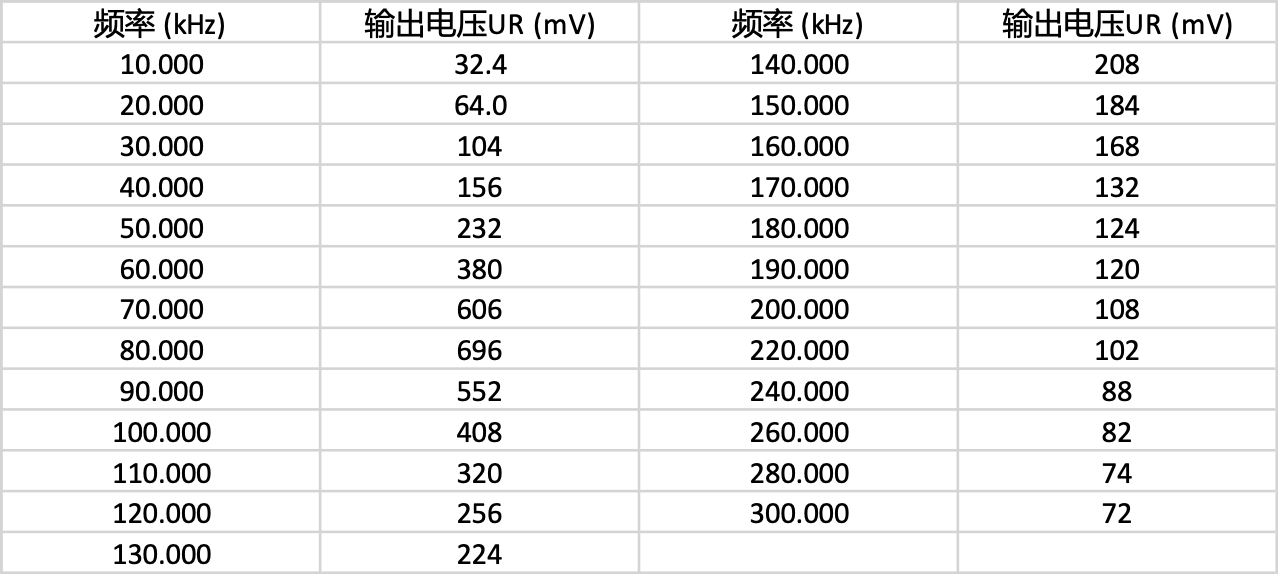
\includegraphics[width=1.0\textwidth]{1-1.png}
    \caption{不同频率下电阻R上的输出电压}
\end{figure}

用平滑曲线连接各个数据点得到谐振曲线如下:

取$U_R = \frac{U_{R_{max}}}{\sqrt{2}}$,得到半功率电频率$v_1$和$v_2$,计算与与光滑曲线的交点。

实现代码如下:

\begin{python}
import numpy as np
import matplotlib.pyplot as plt
from scipy.interpolate import make_interp_spline
from scipy.optimize import fsolve

x = np.array([10,20,30,40,50,60,70,80,90,100,110,120,130,140,150,160,170,180,190,200,220,240,260,280,300])
y = np.array([32.4,64,104,156,232,380,606,696,552,408,320,256,224,208,184,168,132,124,120,108,102,88,82,74,72])
x_smooth = np.linspace(x.min(), x.max(), 500)
spl = make_interp_spline(x, y, k=3)
y_smooth = spl(x_smooth)

max_y = np.max(y_smooth)
max_x = x_smooth[np.argmax(y_smooth)]
level = max_y / np.sqrt(2)

def find_intersections(x_smooth, y_smooth, level):
    intersections = []
    for i in range(len(x_smooth) - 1):
        if (y_smooth[i] - level) * (y_smooth[i + 1] - level) < 0:
            x_intersect = fsolve(lambda x: spl(x) - level, x_smooth[i])
            intersections.append(x_intersect[0])
    return intersections
intersections = find_intersections(x_smooth, y_smooth, level)

plt.plot(x_smooth, y_smooth, label='Smooth Curve')
plt.plot(max_x, max_y, 'ro', label='Maximum Point')
plt.axhline(level, color='r', linestyle='--', label=f'y = {level:.2f}')
for intersect in intersections:
    plt.plot(intersect, level, 'go')
plt.legend()
plt.show()

print("Maximum point: (", max_x, ",", max_y, ")")
print("Intersections with level line:", intersections)
\end{python}

\newpage

\begin{figure}[htbp]
    \centering
    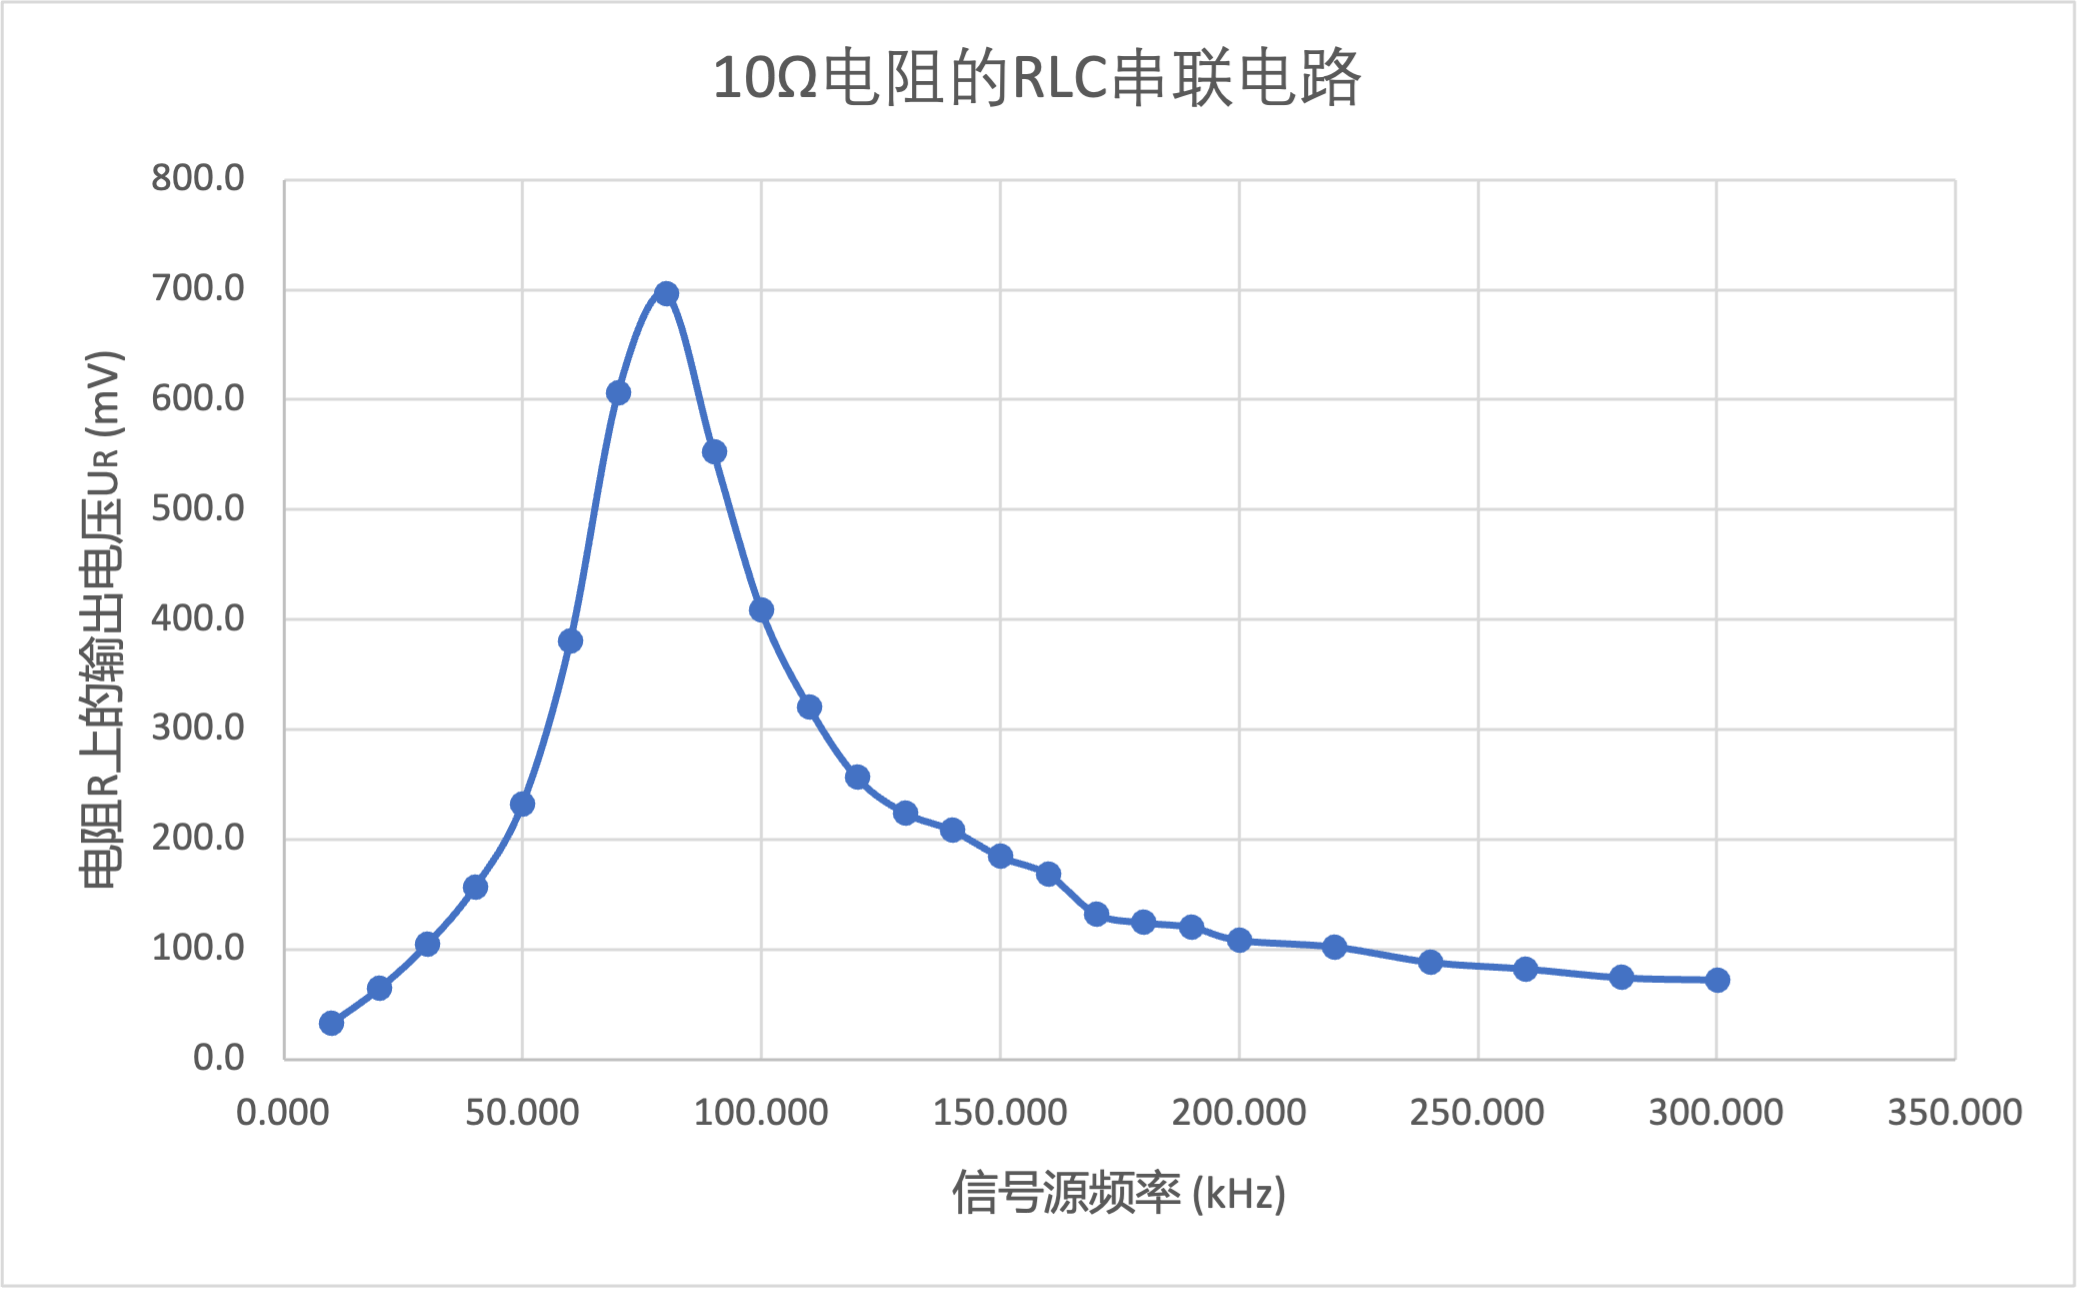
\includegraphics[width=1.0\textwidth]{1-2.png}
    \caption{$10\Omega$电阻的RLC串联电路}
\end{figure}

\begin{figure}[htbp]
    \centering
    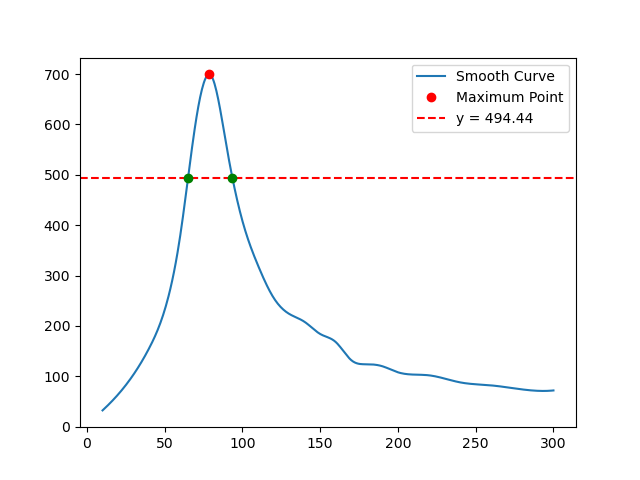
\includegraphics[width=1.0\textwidth]{1-3.png}
    \caption{半功率频率点}
\end{figure}

得到半功率频率点为$(65.014, 494.44), (93.481, 494.44)$,最大值点为$(78.577, 699.238)$

故$v_1 = 65.914 kHz, v_2 = 93.481 kHz, v_0 = 78.577 kHz$

谐振频率可写作为:$v_0 = \frac{1}{2\pi \sqrt{LC}}$

该RLC电路中,$L = 0.1 mH, C = 0.047\mu F$,可以计算得$v_0 = 73.412 kHz$

实验值的误差为:
\begin{equation*}
    \delta = \frac{78.577 - 73.412}{73.412} = +7.04\%
\end{equation*}

\subsection{计算损耗电阻阻值}
对于谐振频率点的$U_i$和$U_R$,有
\begin{equation*}
    \frac{U_i}{R + R_L} = \frac{U_R}{R}
\end{equation*}

故损耗电阻阻值有:
\begin{equation*}
    R_L = \frac{U_i R}{U_R} - R_L
\end{equation*}

实验中,$U_i = 1.00V, U_R = 699.238 mV, R = 10\Omega$,得到$R_L = 4.30 \Omega$

\subsection{计算品质因素}
Q值表征电路选频性能的优劣,也可以标志电路中储存能量与每个周期内消耗能量之比,将两个Q值分别记为$Q_1, Q_2$
\begin{align*}
    Q_1 &= \frac{v_0}{v_2 - v_1} = 2.85 \\
    Q_2 &= \frac{\omega_0 L}{R + R_L} = \frac{2\pi v_0 L}{R + R_L} = 3.45
\end{align*}

\section{改变电阻阻值再次测量RLC串联谐振谐振曲线}
\subsection{测量谐振曲线}
选取$R = 100 \Omega$,连接RLC串联电路,先固定信号源输出电压为$1.00V$,随后将示波器切换到XY模式(李萨如图形),调节信号源频率,直到示波器上出现一条直线,此时找到RLC电路的谐振频率为$v_0 = 80.000 kHz$。

将示波器切换到YT模式,调节信号源输出电压,直到示波器上显示整个电路两端的电压为$U_i = 1.00V$,记录电阻R的输出电压$U_R = 960 mV$

之后,改变信号源的频率,每次调节频率后,都需通过调整信号源输出电压,使得示波器上显示整个电路两端的电压为$U_i= 1.00V$,然后记录电阻R的输出电压,得到数据如下:
\begin{figure}[htbp]
    \centering
    
\includegraphics[width=1.0\textwidth]{2-1.png}
    \caption{不同频率下电阻R上的输出电压}
\end{figure}

用平滑曲线连接各个数据点得到谐振曲线如下:
\begin{figure}[htbp]
    \centering
    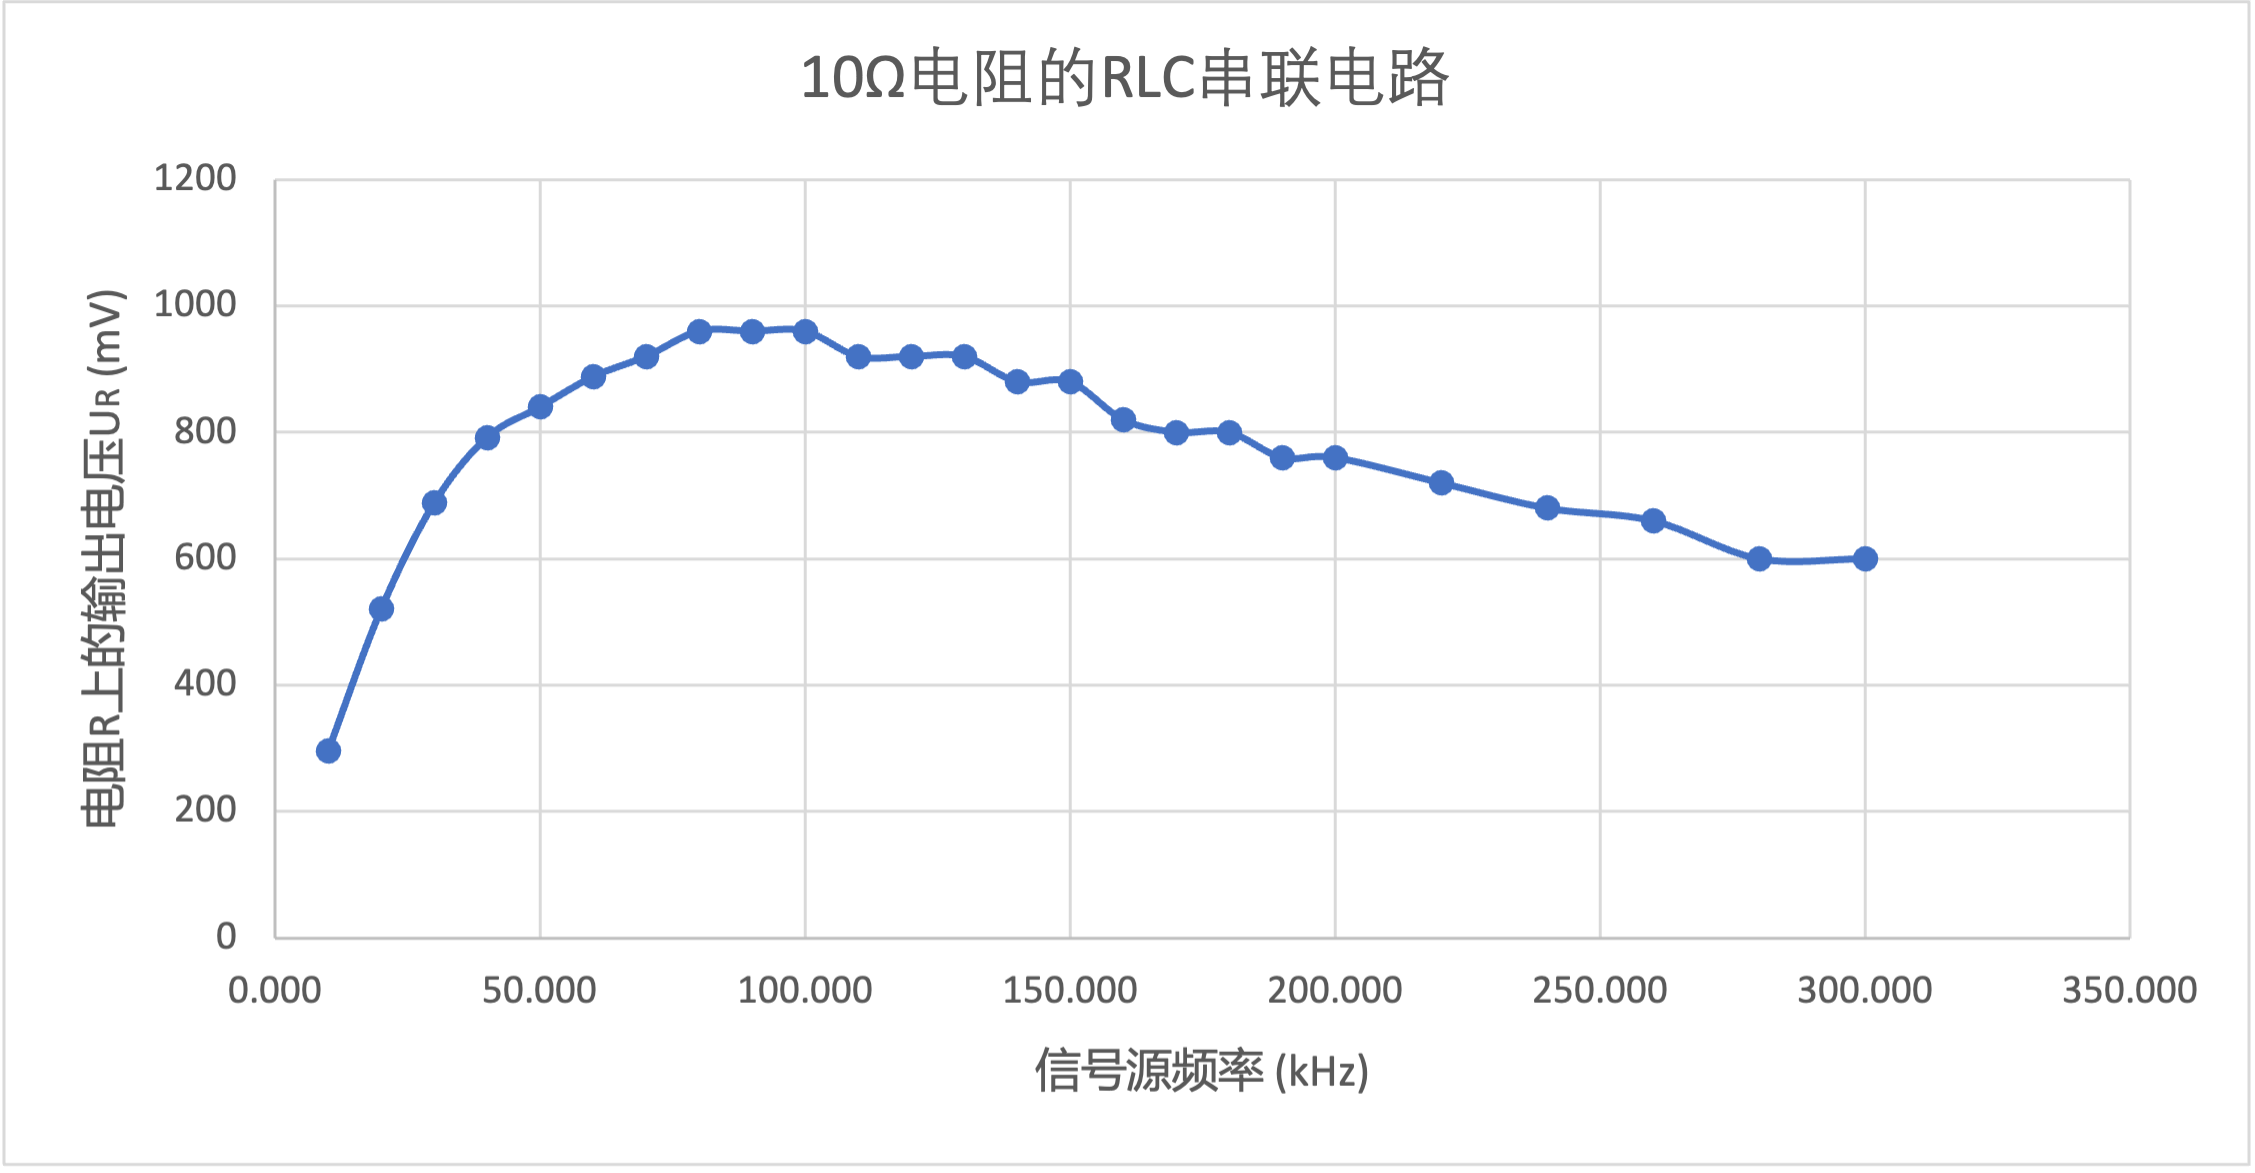
\includegraphics[width=1.0\textwidth]{2-2.png}
    \caption{$100\Omega$电阻的RLC串联电路}
\end{figure}

实现代码同上,只更改了添加实验数据点的部分(如下):
\begin{python}
x = np.array([10,20,30,40,50,60,70,80,90,100,110,120,130,140,150,160,170,180,190,200,220,240,260,280,300])
y = np.array([296,520,688,792,840,888,920,960,960,960,920,920,920,880,880,820,800,800,760,760,720,680,660,600,600])
\end{python}

取$U_R = \frac{U_{R_{max}}}{\sqrt{2}}$,得到半功率电频率$v_1$和$v_2$,计算与与光滑曲线的交点。
\begin{figure}[htbp]
    \centering
    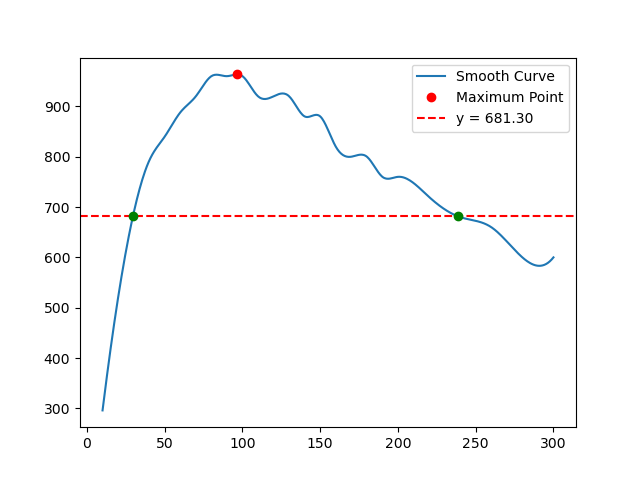
\includegraphics[width=1.0\textwidth]{2-3.png}
    \caption{半功率频率点}
\end{figure}

得到半功率频率点为$(29.519, 681.30), (238.812, 681.30)$,最大值点为$(96.593, 963.508)$

故$v_1 = 29.519 kHz, v_2 = 238.812 kHz, v_0 = 96.593 kHz$

根据前一部分,可以计算得$v_0 = 96.593 kHz$

实验值的误差为:
\begin{equation*}
    \delta = \frac{96.593 - 73.412}{73.412} = +31.58\%
\end{equation*}

\subsection{计算损耗电阻阻值}
损耗电阻阻值有:
\begin{equation*}
    R_L = \frac{U_i R}{U_R} - R_L
\end{equation*}

实验中,$U_i = 1.00V, U_R = 963.508 mV, R = 100\Omega$,得到$R_L = 3.79 \Omega$

\subsection{计算品质因素}
Q值表征电路选频性能的优劣,也可以标志电路中储存能量与每个周期内消耗能量之比,将两个Q值分别记为$Q_1, Q_2$
\begin{align*}
    Q_1 &= \frac{v_0}{v_2 - v_1} = 0.46 \\
    Q_2 &= \frac{\omega_0 L}{R + R_L} = \frac{2\pi v_0 L}{R + R_L} = 0.58
\end{align*}

\section{分析与讨论}
1. 理论谐振频率与实验测量谐振频率的误差分析
\begin{itemize}
    \item 实际电感和电容器的标称值可能与其真实值存在偏差。温度变化对电感和电容值的影响可能导致谐振频率的偏移。
    \item 频率的测量和示波器的读数精度也会影响结果,例如频率调节的精度有限,示波器的分辨率也是有限的。
    \item 在实际情况中,电感线圈的电阻以及电容的漏电阻都会影响谐振频率,导致测量值与理论值不一致。
    \item 本实验中,$7\%$左右的误差由于上述原因造成,在可以接受的范围内。
\end{itemize}

2. 两种方法计算品质因素Q得到的结果不同
\begin{itemize}
    \item 根据频带宽度计算的$Q_1$,测量的精度和曲线拟合的准确性会直接影响计算结果。若谐振曲线的两侧不对称或测量数据有误差,都会导致Q值计算不准确。在取$R=100\Omega$时,谐振曲线两侧尤其不对称。
    \item 根据电路中各个参数计算的$Q_2$,在理论上是准确的,然而实际电路中的损耗电阻$R_L$以及其他非理想因素也会影响计算结果。
\end{itemize}

3. 选取不同的$R (10\Omega, 100\Omega)$导致的差异
\begin{itemize}
    \item 电阻R的大小直接影响谐振曲线的形状。较大的电阻会使谐振曲线变得平缓,谐振频率偏移更明显,Q值变小;较小的电阻则会使谐振曲线更尖锐,Q值较大。
    \item 实际应用中,如果需要更高的Q值(更好的选频性能),则需要选择阻值较小的电阻;如果对电路的稳定性和功率损耗有较高要求,则需要权衡选择适中的电阻值。
\end{itemize}

4. 该实验中整体的误差来源
\begin{itemize}
    \item 系统误差:电感、电容和电阻的标称值与实际值之间的差异
    \item 随机误差:信号源输出频率和电压的精度,示波器的测量精度和读数误差
    \item 测量误差:信号源输出的不稳定性
\end{itemize}

\end{document}